\chapter{Conclusion and Future Work}
\section{Conclusion}
The goal of this project was to introduce new intermediary service providers and replace the ID-centric append-only log from Secure Scuttlebutt with a feed bundle protocol. This extension or modification allows a much easier onboarding experience, since the client is indirectly connected to all the ISP's servers after signing a contract with an ISP. With the new introduce-detruce architecture, clients can connect and diconnect to new servers in a simple manner. Within this process new feed pairs are created, which bundle all the information for that specific connection. To ease the load on the wire and the process of replicating every feed through the ISP directly to the server, requests are multiplexed into a single feed pair between the ISP and the Server.
Since this system is so new an has been developed completely "out of the blue", there are many ways to improve it, one of which is to use the feeds properties primarily to define the state of doneness inside the single log entries. There are still many avenues to be explored and important key features to be added to in order to generate relieable Client-ISP-Server Network, some of which are discussed within the next section.

\section{Future Work}
Apart from improving the general system, we have only examined the connection between a single ISP with a single connectivity node with a random number of clients and servers connected. In the real world, however,  this is not the case. There are many ISPs on the market which have connectivity stations all over their respective countries. Therefore internet service providers (ISPs) and internet connectivity providers (ICPs) can be separated. Contracts between two ISPs would also be conceivable. In the process of creating the simplified version of the feed bundle protocol, we always kept the big picture in the foreground and decisions were made keeping this in mind.

\section{Combination of Log Entries}
Seen in the concept and the implementation, only a single new log entry is multiplexed into the ISP-server feed pair, resulting in a replication after each request. A diffrent approach can be made. We combine log entries in the multiplexing system. Meaning, instead of only one, a defined number of new log entries will be multiplexed to the server. This gives room for more efficient replication, since the whole feed gets replicated to the peer every time. Deriving from this the multiplexing feed pair can be splited up into arbitrary many sub feed pairs, linked to the priority of the request. 
\section{ISPs and ICPs}
As mentioned previously, the ISP was always a single node, with contracts to clients and servers. However, we could also look at the ISP as a company with a network of ICPs where the physical connection between the servers and clients takes place. In simple terms, the client and server were indirectly ’connected’ through the ISP. The initial concept of this thesis was a peer-to-peer Internet Connectivity Provider (ICP) network where the ISP-Company distributes the feeds internally between the ICPs. In real life, there is a contract with the ISP, e.g. Swisscom, and this same ISP has connectivity provider stations or nodes within the ISP network of ICPs. This means that a client has a connection to icp342 of Swisscom and the server has a contract with icp903. But both have a contract with Swisscom, which provides internal routing to pass information from icp342 to icp903.
\begin{figure}
    \centering
    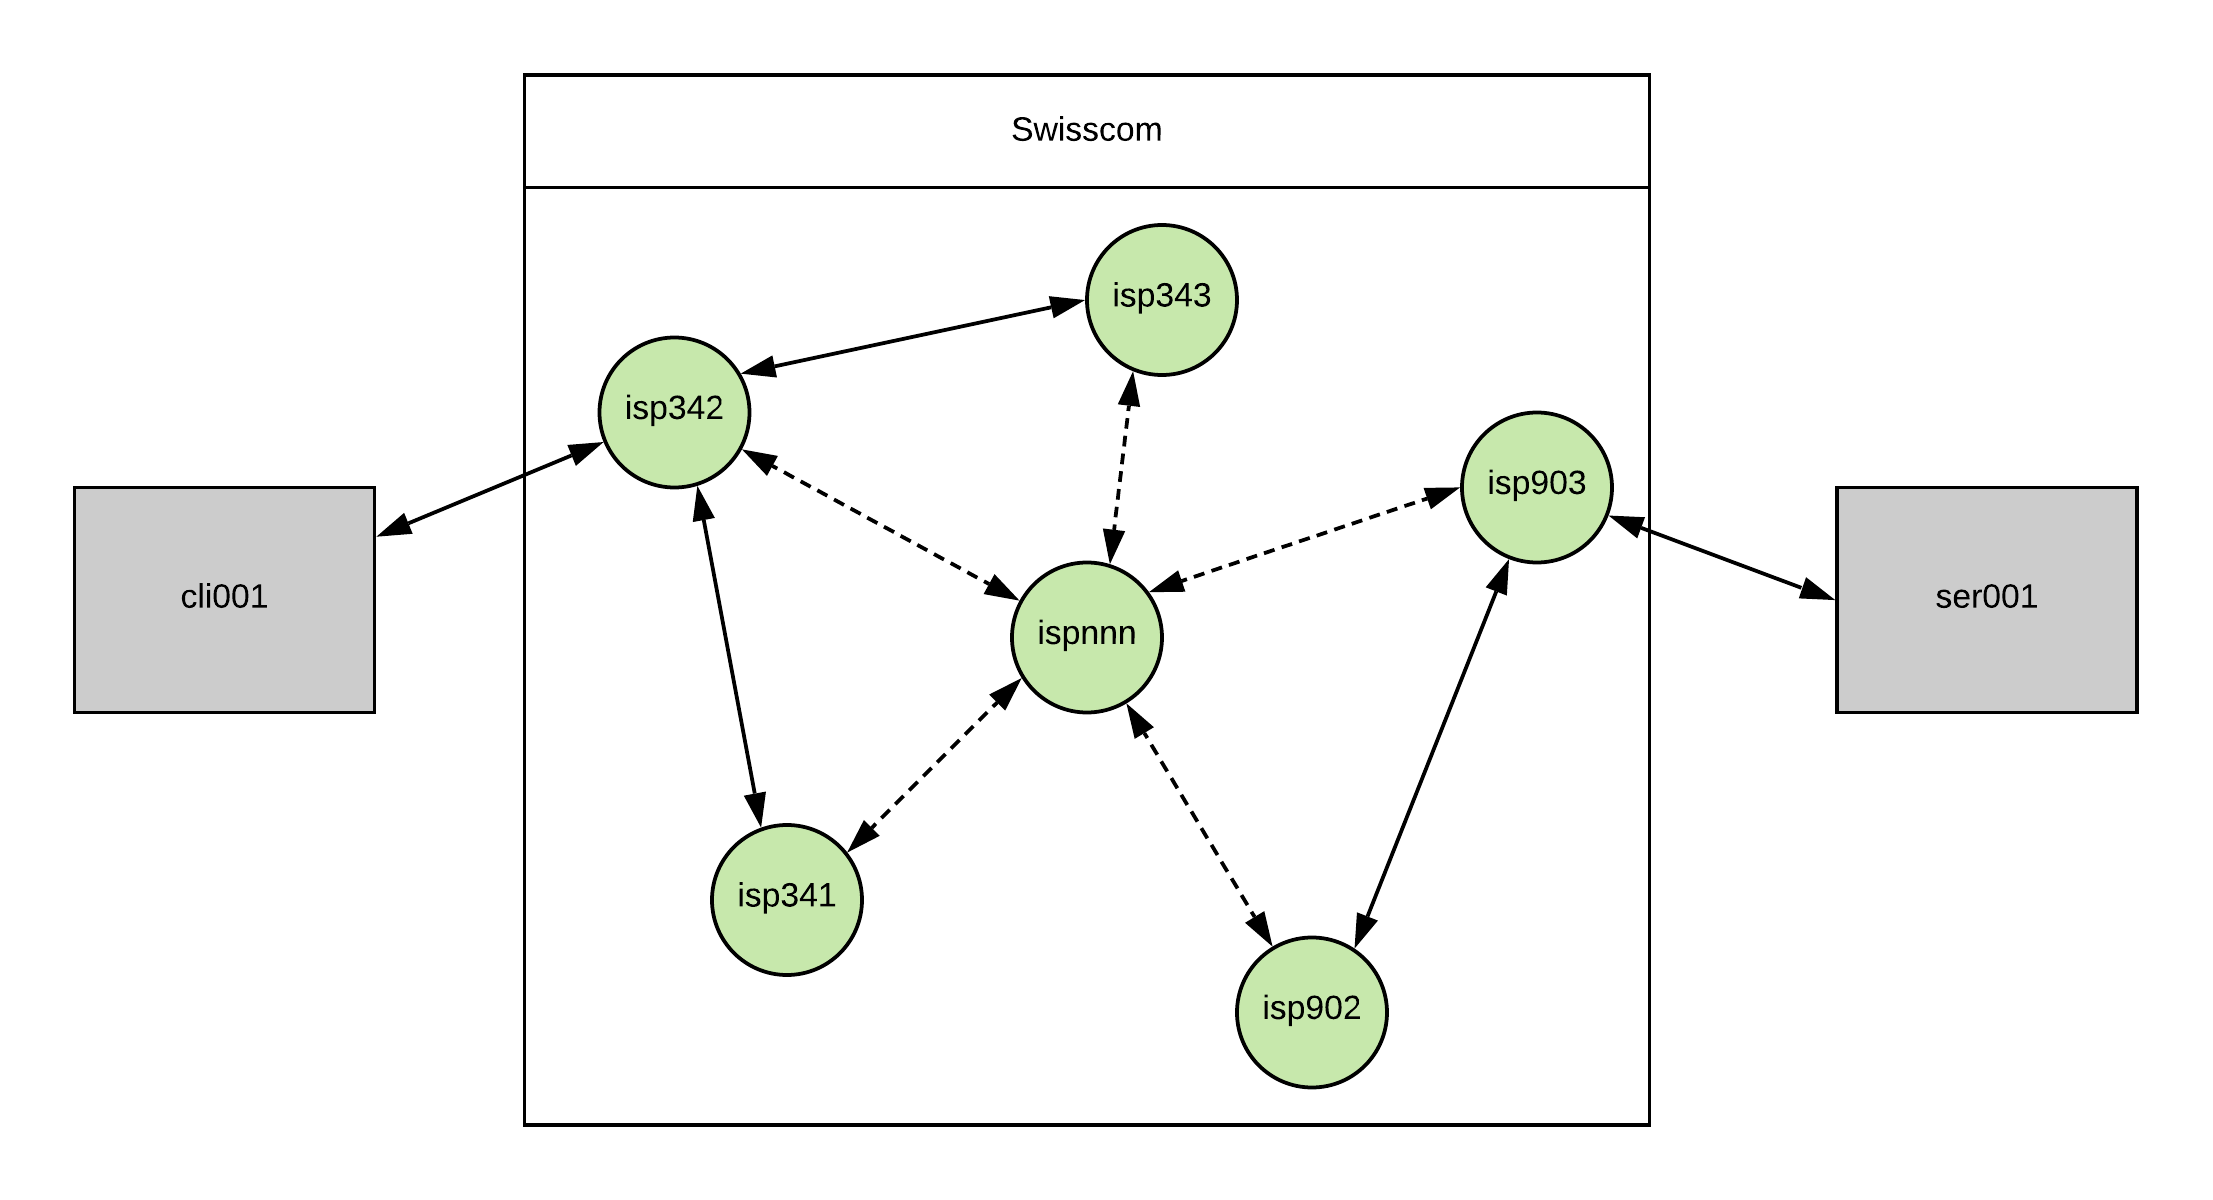
\includegraphics[width=0.9\textwidth]{p2p_contracts}
    \caption{A simplified contract network.}
    \label{fig:contract_network}
\end{figure}
In light of this fact, a new challenge emerges. How are the feeds replicated? Either with the same approach as is currently the case, where every ICP node stores a replication of each feed-pair which it routes to the next node, or only by appending the multiplexed log entries to the ICP-ICP feed-pair. Additionally,  it should be possible for a client to change the connectivity provider, for example when traveling from Basel to Zurich. In this case, the ICP will change, since it routes to antennas in the respective cities. New algorithms need to be developed tho handle exactly such use cases.

\section{Contracts between ISPs}
Yet again, we can take this distribution to the next level where ISPs have contracts with other ISPs. This provides a way to bypass the current requirement that each ISP must have a contract with each server. This has a very special impact on the system however, since new contracts are generated, when the business aspect hase not yet been defined. This problem is more easily explained with an example.\\
\textit{rewrite}
If we say Google has a contract with Swisscom and Sunrise wants to have a contract to Google. There will be some money involved. Let's say Google pays Swisscom a hundred swiss francs for every introduced client. So Google has now the opportunity to make a contract with Sunrise, but they do not like each other very much and had difficulties earlier. So Google offers Sunrise fifty swiss francs per connected client. So Sunrise probably will not sign, since they have a good relationship with Swisscom. So now Swisscom offers Sunrise 75 swiss francs for every client they provide to Google. Now you see the dilemma. In the first scenario Google would make more profit, where as the second scenario is better for Swisscom and Sunrise. These dynamics are not simple, hence very interesting and have to be clarified. 
